\chapter{Introduction}

\section{Project group}
The bachelor group consists of the following four IT students:
\begin{itemize}
    \item Andreas Harnes. 
    Computer Science student with interests in networking and programming.
    \item Celina Marie Kristiansen.
    Computer Science student with experience in databases and big data.
    She has previously been deployed at Logiq where she used Databricks to process data.
    \item Magnus Klerck.
    Information systems student with background as a computer electrician where he worked with IT maintenance and hardware repair.
    He also has an interest in cybersecurity.
    \item Morten Offerdal Kvigne.
    Computer Science student with interests in programming and data security.
\end{itemize}
Celina M. Kristiansen, Magnus Klerck and Morten Offerdal Kvigne have previously been working on projects together.
The three had effective collaborations in their former projects which is reflected in the results they produced.
Due to the effective collaboration the three of them decided to form this bachelor group.

Magnus and Morten had both previously worked with Andreas Harnes and they both believed him to be knowledgeable and as such he was brought in.

\section{Assignment provider}
MakerSpace is a workspace at Østfold University College in Halden. 
The workspace acts as a playground for students and employees who like to use technology to create something.
MakerSpace is operated by Michael Andersen Lundsveen and 4 student assistants but all students and employees at Østfold University College have access to the facility 24 hours, 7 days a week
\cite{what-is-makerspace}.
Østfold University College describes the drive behind MakerSpace as:

\begin{displayquote}
The purpose of Makerspace is to offer students a physical space and an engaging environment with the aim to learn something new by encouraging curiosity and eagerness.
\end{displayquote}
In addition MakerSpace also acts as an area for lectures, courses and experiments.
They also hold basic programming courses for children during the summer.

MakerSpace is equipped with various equipment related to several fields.
Some of the equipment MakerSpace offers is 3D printers, which can be used to print out different figures and shapes in plastic from a 3D model. Soldering irons for making circuits and soldering components, computers with VR headsets, lego robots and remote controlled drones as shown in fig.1\cite{Figure-Drone}. MakerSpace also has different tools like screwdrivers, workbenches, pliers, RJ45 crimpers to mention some.

Lastly MakerSpace allows students and employees at Østfold University College to borrow equipment.
Students and employees have to note down their name, their contact information and the item(s) they are lending in a book used to keep track of all borrowed equipment whenever they are borrowing equipment.

MakerSpace responsible Michael Andersen Lundsveen is the assignment provider for the project. 
Michael is the leader and principal engineer for MakerSpace Halden.
He oversees day to day operations and he ensures all equipment is in good condition.
Additionally he is responsible for the repairment or the purchase of new equipment should equipment be damaged or destroyed.
Michael also arranges courses for the MakerSpace employees allowing them to learn how to utilize new equipment, he arranges summer workshops for children during the summer vacations and he sponsors certain arrangements and events at Halden University College.

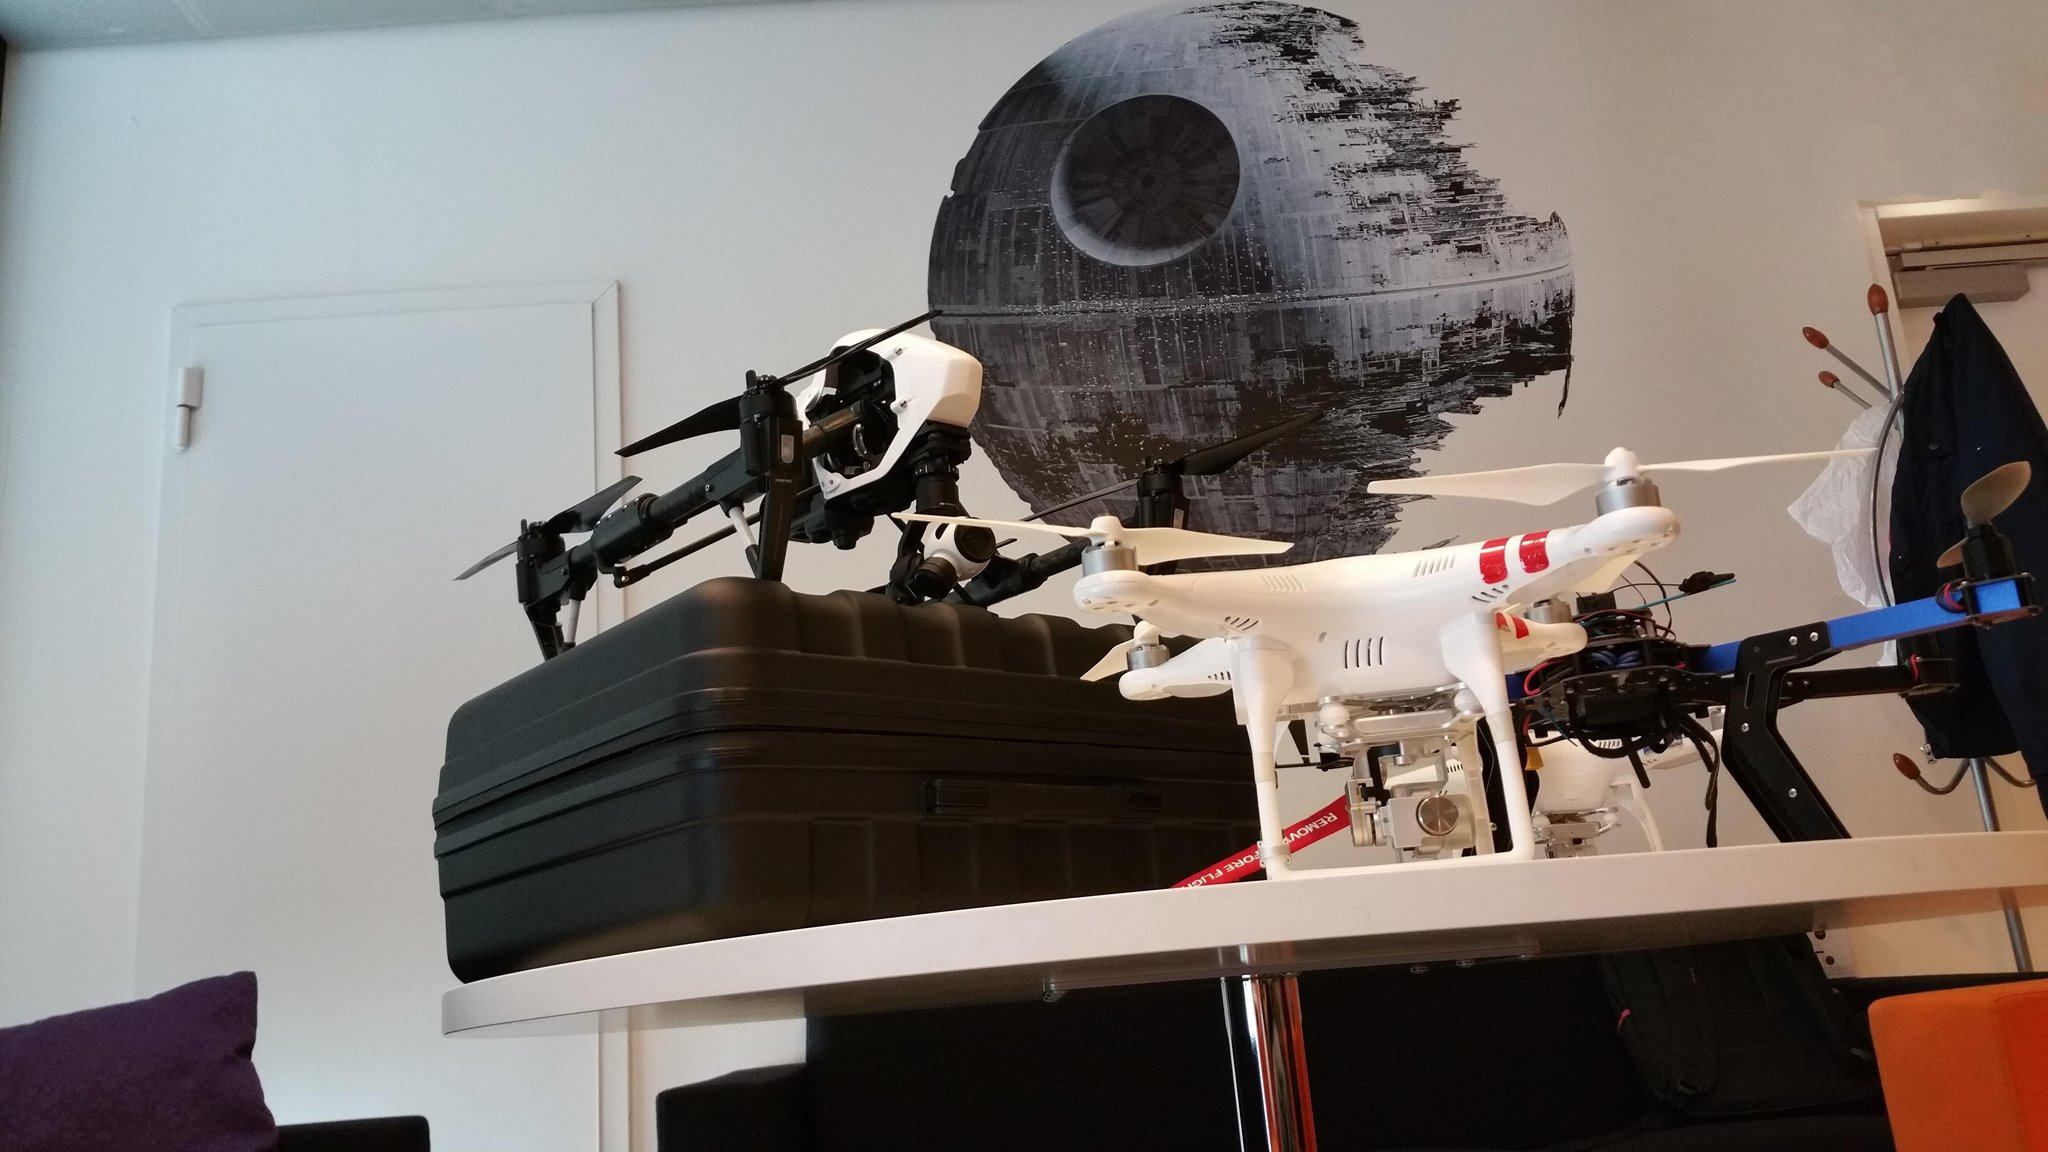
\includegraphics[width=115mm,scale=1]{images/makerspace.png}

\section{The mission}
The background for the project is that MakerSpace currently does not have an overview of what equipment they have, whether said equipment is available and where said equipment is stored.
This is problematic for the employees at MakerSpace as they have no way of knowing whether equipment is missing or the equipment is damaged.
Even if an employee is made aware of missing or damaged equipment the employee currently has no way of notifying the other employees and as such the employee will have to manually contact the other employees in order to notify them which is hassling.

This is also problematic for the users of MakerSpace.
The users have to search through MakerSpace in its entirety in order to find a given piece of equipment.
They have no way of knowing whether the piece of equipment is damaged until they find it.
They also have no way of knowing whether MakerSpace does not offer said piece of equipment or whether another user is currently borrowing it should they not find it.

Lastly the book used when borrowing equipment also proves problematic.
Anyone can inspect the contents of the book and as such the book does not respect the privacy of the users.
This is especially concerning should the book be stolen.
Additionally the book can disappear.
Finally the book is not protected in the event of a fire.

%\todo{Hva ønsker dei forskjellige brukerene av systemet; hva ønsker dei som jobber der, hva ønsker dei som skal låne utstyret?}
%At the moment there is no written overview of equipment and tools on MakerSpace. All information about the equipment and tools there is what the student assistants know and can help find. When there are no student assistants in MakerSpace, there is no way to find out if MakerSpace has the equipment or tool you need. There is an analogue system for lending. A book is used where all of the loaned equipment is written down. This system has proven not to work properly as students and employees do not use the system for lending.

In order to solve the issues outlined above the group intends to develop two modules.
The employees and users will interact with the modules using web pages.
The following two modules will be developed:
\begin{itemize}
    \item An inventory module allowing employees and users to view the equipment MakerSpace offers, the equipment's condition, where the equipment is stored and weather the equipment is available.
    The module will also allow employees to add, modify and delete equipment from the module.
    \item A lending module allowing employees and users to borrow equipment.
    When returning equipment the module also allows the employee or the user to report any damage that occurred whilst the equipment was being borrowed.
\end{itemize}

The modules will be extendable.
This allows future features to be incorporated into the modules without difficulties for future developers.

%What MakerSpace wants is a system that gives Michael and student assistants access to an overview of all the equipment and tools available in MakerSpace. This system must be modular so that it can be further developed later, and in addition to this a inventory system. They also want a lending module that makes it easier to register the lending of equipment and tools.

%What the group is planning to develop is a modular inventory system and a lending module by adopting technology that is in use today.

%\todo{TODO Alt under flyttes til metode}
%\textbf{Investigation:} The group have talked about some technology they could potentially use. Some of the technology the group have been thinking about is: Vue.js, Node.js and MongoDB. The group will do a investigation for each of those and find out if they fit the project or not. The group will also try and find other technologies that can be more applicable for the project.

%\textbf{Development:} The group will create a website that will offer a lending system of equipment that exists at MakerSpace and also make sure that the system can be further developed later on.

%In the development of the system, the group have made some bullet-points as an overview for the project. These are:
%\begin{enumerate}
%  \item Make the website that will be used for the system and make sure it follow the criteria for universal design.
%  \item Design a structure for the inventory storage.
%  \item Make a module for lending.
%  \item User test the system to find bugs.
%\end{enumerate}

\section{Purposes, delivery and method}
\subsection{Purposes}
%There are two reasons for the project.
%The first is to provide an overview of the equipment available at MakerSpace to the employees and users of MakerSpace.
%This is beneficial as the employees and users now no longer need to search through MakerSpace in its entirety to see if MakerSpace offers the equipment they seek.

%The second reason is to digitize the lending system MakerSpace currently has in place.
%This is beneficial because it is privacy respecting as only those with the necessary permissions can view the records of equipment currently being borrowed. 
%Additionally should equipment not be returned MakerSpace will know who is responsible.
%Lastly the records of borrowed equipment can be place on a backup - meaning the records of borrowed equipment are not lost in case of theft or in case of a fire.

\textbf{Main goal:} Make an inventory module which provides an overview of the equipment available at MakerSpace.

\textbf{Sub goal 1:} Make a lending module which digitizes the current lending system used at MakerSpace.

%The purposes with this project is to digitize the current lending system. This will make it easier to not only see what equipment that is available for lending but also what equipment that needs to be order more of. This is divided into a main goal and some sub-goal's.

%\textbf{Main goal:} Digitize current lending system and write the report.

%\textbf{Sub-goal 1:} Make a inventory structure with a lending module

%\textbf{Sub-goal 2:} Make sure that the website (e.g front-end, UI,UX) follow the criteria for universal design.

\subsection{Delivery}
%Here comes a list of what the group is going to deliver for this project. Alongside with the delivery of an lending system, the group also need to deliver some documentation and a main report.

Below are the deliveries the group will deliver during the project.%\todo{Legge på lending module/inventory module?}

\begin{tabu} to 1.2\textwidth { | X[l] | X[c] | }
    \hline
    \textbf{Date} & \textbf{Delivery} \\
    \hline
    January 18 ,2019 & Pilot report \\
    \hline
    March 08, 2019 & First version of main document \\
    \hline
    April 23, 2019 & Second version of main document \\
    \hline
    April 26, 2019 & Product \\
    \hline
    May 16, 2019 & Finished version of main document \\
    \hline
    May 27, 2019 & Project poster \\
    \hline
   June 03, 2019 - June 05, 2019 & Presentation of the project \\
    \hline
    \end{tabu}
    
\subsection{Method}
The group has decided to use an agile model for the software development process.
The project is small in scale and is not tightly integrated with any other system.
This means the comprehensive documentation a waterfall model requires is not needed.
Additionally this means informal communications between group members work well as the group is co-located.
The agile model does however require a higher presence of the assignment provider as he plays an integral part in which components the group are to prioritize.

The assignment provider is involved and accessible throughout the project development.
This allows for incremental development of the requirements set out by the assignment provider which means contract negotiations are not necessary.
Consequently the group can more easily adapt to changes in requirements as the documentation remains largely unaffected by the respective changes.
This is the driving factor behind the agile model:
\begin{displayquote}
Agile is the ability to create and respond to change.
It is a way of dealing with, and ultimately succeeding in, an uncertain and turbulent environment \cite{what-is-agile}.
\end{displayquote}
This is also one of the factors which separates the agile model approach to that of other software development models:

\begin{displayquote}
One thing that separates Agile from other approaches to software development is the focus on the people doing the work and how they work together.
Solutions evolve through collaboration between self-organizing cross-functional teams utilizing the appropriate practices for their context \cite{what-is-agile-software-development}.
\end{displayquote}
With everything taken into consideration the group believes an agile model is more suited for this project than that of a waterfall model.

The group believes the best way to organize the project is using the agile framework Scrum.
Scrum is a framework that is best suited for teams with a size of seven or less \cite{software-engineering-scrum-size} which makes the framework ideal for the group as the group consists of four members.
The assignment provider has set forth the features he would like to see in the system and these features make up the product backlog.
Given the fact that the assignment provider is so involved and accessible it seems fitting that he is involved in deciding which functionality is to be prioritized which Scrum allows him to do as a product owner.
The group believes the flexible approach an agile model used through Scrum provides the best foundation for the successful completion of the project.

%SCRUM (source: https://www.mountaingoatsoftware.com/agile/scrum) will be used as a framework to manage the project and the software development. SCRUM is a derivative of the Agile methodology, but we will use Agile (source:https://www.agilealliance.org) as the methodology when developing software for the project. The Agile method will be used so the group can adjust and adapt to changes in the development as the project goes along. By scaling this to the scope of the group and the project, Agile will fit the development of the project well. 

 When working on the report and documentation for the project it will follow qualitative research methods for gathering information and comparing/analyzing data. Qualitative research method is a scientific method of observation to gather non-numerical data. The aim of a qualitative research project may vary with the disciplinary background, like a mechanical engineer seeking in-depth understanding of a combustion engine for example.
 
 Qualitative methods are best for researching many of the why and how questions of something \cite{Qualitative-Research}. Qualitative research is widely used by political science, social work, and education researchers and only produce an explanation for the particular case that is studied. All the qualitative research done for this project will be focused on how we will do something and why that is the best way to do it. Like why did the group choose a certain program over another and how we are going to use said program. The reason for this is that the project does not need any quantitative data for the documentation of the project, one exception that might occur is in the testing phase. In the testing phase the project group will ask for a number of students and/or employees to test the developed system and it's ease of use i.g: UI, UE and possible bugs. The data collected from testing could be used to statistically to show that the UI and UX is good for all potential users. No matter how experienced the users are with IT or how many times the users have used the system.

\section{Report structure}

\textbf{Chapter 1, Introduction:}
Gives background information about the project as well as a brief summary of the methodology used.

\textbf{Chapter 2, Analysis:}
Provides a thorough description of the assignment based on the requirements set by the assignment provider in addition to explaining what the selected technologies are and why they are suitable for the project.

\textbf{Chapter 3, Design, form and planning:}
Explains how the components of the application are designed and how these components are intended to connect to form the final application.

\textbf{Chapter 4, Implementation:}
Describes how the application was built and which tools were used in doing so in addition to a description of the application itself.

\textbf{Chapter 5, Testing and Evaluation:}
Explains how the components of the application were tested - which components were tested, how were they tested and who tested them.
The chapter also provides the feedback received and whether the application passed the acceptance tests.

\textbf{Chapter 6, Discussion:}
Describes the project process - what went well, what did not and what could have been done differently.
The chapter also outlines what the group has learned during the project.

\textbf{Chapter 7, Conclusion:}
Presents the results and outlines the continuation of the project.

%\todo{Bør leses over og rettskrives}In chapter 2 the group will go more in to details of the requirements for both the academic and technical documents. 

%Then in chapter 3 we will go more into the structure, the content and the design of the program that the group will make. Here we will explain the design choices the group made in the front-end user interface, the structure of the database and the design of the api calls.

%In the fourth chapter we will write more about how the group implemented the different technologies the group will use in the different parts of the project and what other technology choices that could have been done instead.

%The fifth chapter will contain most of the documentation about the testing done on the system, and how the system was tested. Here the feedback given by the product testers and product manager will be documented.

%The focus of the sixth chapter will be more about how the group experienced the project and what was learned by doing it. Here it will also be documented what could have been done differently and what worked well.

%The seventh chapter will contain the groups conclusion of the project. Here all the important scientific discoveries will be documented and described such that any reader can read this part of the document and now what the rest is about.
